\subsubsection{\texorpdfstring{\ding{224} General layout}{General layout}}%\vspace{6pt}%
%%%%%%%%%%%%%%%%%%%%%%%%%%%%%%%%%%%%%%%%%%%%%%%%%%%%%%%%%%%%
% Z list
\label{option_Z list}%
\pgfPTMoption{4}{Z list}{all}%
{Set's the list of the elements to display in the Periodic Table. It could be a \lblue{name} or a \lblue{comma sepa\-rated} list of atomic numbers, which in turn supports \textit{the dots notation} as explained in the section \textit{Repeating Things: The Foreach Statement} in the \href{https://www.ctan.org/pkg/pgf}{pgfmanual}.}
\\ [5pt]\pgfPTMmacrobox{pgfPT}[Z list={1,...,36}]%
\\ [5pt]\makebox[\linewidth][c]{\scalebox{.6}{\pgfPT[Z list={1,...,36}]}}%
\\ [10pt]\pgfPTMoptiontxt{%
The possible \lblue{name} is one of the following:
\begin{itembar}
\item\textbf{built-in}:
\begin{itemize}
\item[\raisebox{1pt}{\scriptsize$\vartriangleright\,$}]\sq{all} is equivalent to \green{Z list=\{1,...,118\}}, \ie, all known elements.
\item[\raisebox{1pt}{\scriptsize$\vartriangleright\,$}]\sq{s}, \sq{p}, \sq{d} or \sq{f}, for the elements in the corresponding blocks.
\item[\raisebox{1pt}{\scriptsize$\vartriangleright\,$}]\sq{sp}, \sq{spd}, for the elements resulting from merging the corresponding blocks.
\item[\raisebox{1pt}{\scriptsize$\vartriangleright\,$}]\sq{lanthanoids} or simply \sq{La}, for lanthanoids\red{$\,^\dag$}.
\item[\raisebox{1pt}{\scriptsize$\vartriangleright\,$}]\sq{actinoids} or \sq{Ac}, for actinoids\red{$\,^\dag$}.
\item[\raisebox{1pt}{\scriptsize$\vartriangleright\,$}]\sq{G1*}, \sq{G1}, \myldots\ , \sq{G18}, which are used, respectively, for the elements of \textit{group 1 without hydrogen}, \textit{group 1}, \myldots\ , \textit{group 18}.
\item[\raisebox{1pt}{\scriptsize$\vartriangleright\,$}]\sq{ P1}, \myldots\ , \sq{P7}, \sq{P6*}, \sq{P7*}, which are used, respectively, for the elements of the \textit{1\raisebox{3pt}{\scriptsize st} period}, \myldots\ , \textit{7\raisebox{3pt}{\scriptsize\hspace{.5pt}th} period}, \textit{6\raisebox{3.5pt}{\scriptsize\hspace{.25pt}th} period and lanthanoids}\red{$\,^\dag$}, \textit{7\raisebox{3pt}{\scriptsize\hspace{.5pt}th} period and actinoids}\red{$\,^\dag$}.
\\ [3pt]\makebox[\linewidth][r]{\scriptsize\red{$^\dag\,$}\textit{Depending on the value of the \red{IUPAC} key, the Lanthanum or Actinium are or are not included}.}
\end{itemize}
\item
any \textbf{user defined} name via \pgfPTMmacro{pgfPTnewZlist}[]\{name\}\{list\}
\end{itembar}%
}%
\\ [-10pt]\pgfPTendoption%
\newpage\vspace{-34pt}\ %
% cell width
\label{option_cell width}%
\pgfPTMoption{4}{cell width}{34pt}%
{Sets the width of each base cell of the Periodic Table.}%
\\ [5pt]\pgfPTMmacrobox{pgfPT}[Z list={1,...,36},cell width=40pt]%
\\ [10pt]\makebox[\linewidth][c]{\scalebox{.6}{\pgfPT[Z list={1,...,36},cell width=40pt]}}%
\\ [5pt]\pgfPTendoption%
% cell height
\label{option_cell height}%
\pgfPTMoption{4}{cell height}{38.25pt}%
{Sets the height of each base cell of the Periodic Table.}%
\\ [5pt]\pgfPTMmacrobox{pgfPT}[Z list={1,...,36},cell height=50pt]%
\\ [10pt]\makebox[\linewidth][c]{\scalebox{.6}{\pgfPT[Z list={1,...,36},cell height=50pt]}}%
\\ [5pt]\pgfPTendoption%
% cell size (style)
\label{style_cell size}%
\pgfPTMstyle{4}{cell size}{38.25pt}%
{Style to set both the width and the height of each base cell of the Periodic Table.}%
\\ [5pt]\pgfPTMmacrobox{pgfPT}[Z list={1,...,36},cell size=40pt]%
\\ [10pt]\makebox[\linewidth][c]{\scalebox{.6}{\pgfPT[Z list={1,...,36},cell size=40pt]}}%
\\ [5pt]\pgfPTendstyle%
\newpage\vspace{-34pt}\ %
% cell line width
\label{option_cell line width}%
\pgfPTMoption{4}{cell line width}{0.4pt}%
{Sets the width of the line surrounding the base cell of the Periodic Table.}%
\\ [5pt]\pgfPTMmacrobox{pgfPT}[Z list={1,...,36},cell line width=2pt]%
\\ [10pt]\makebox[\linewidth][c]{\scalebox{.6}{\pgfPT[Z list={1,...,36},cell line width=2pt]}}%
\\ [5pt]\pgfPTendoption%
% cell line color
\label{option_cell line color}%
\pgfPTMoption{4}{cell line color}{black}%
{Sets the color of the line surrounding the base cell of the Periodic Table.}%
\\ [5pt]\pgfPTMmacrobox{pgfPT}[Z list={1,...,36},cell line color=red]%
\\ [10pt]\makebox[\linewidth][c]{\scalebox{.6}{\pgfPT[Z list={1,...,36},cell line color=red]}}%
\\ [5pt]\pgfPTendoption%
% cell style
\label{option_cell style}%
\pgfPTMoption{4}{cell style}{\{\}}%
{Loads a named cell style, built via \pgfPTMmacro{pgfPTbuildcellstyle}[], to use as a layout for each cell of the Periodic Table.}%
\\ [5pt]\pgfPTMbuildcellstyle{myname}(5,3)[(1;1-2;Z),(1;3;ls),(2-3;1.5-2.5;CS),(4;1-3;name),(5;1-3;eConfignl)]%
\pgfPTbuildcellstyle{myname}(5,3)[(1;1-2;Z),(1;3;ls),(2-3;1.5-2.5;CS),(4;1-3;name),(5;1-3;eConfignl)]%
\\ [-4pt]\pgfPTMmacrobox{pgfPT}[Z list={1,...,36},cell style=myname]%
\\ [10pt]\makebox[\linewidth][c]{\scalebox{.6}{\pgfPT[Z list={1,...,36},cell style=myname]}}%
\\ [5pt]\pgfPTendoption%
% cell={w=??,h=??,s=??,lw=??,lc=??,style=??} (pseudo style)
\newpage\vspace{-34pt}\ %
\label{style_cell}%
\pgfPTMstyle{4}{cell}{\{w=34pt,h=38.25pt,lw=.4pt,lc=black\}}%
{\textit{Pseudo style} to set the cell \textbf{w}idth, the cell \textbf{h}eight, the cell \textbf{s}ize, the cell \textbf{l}ine \textbf{w}idth, the cell \textbf{l}ine \textbf{c}olor and/or the cell \textbf{style}. None of the \textit{keys} -- w, h, s, lw, lc and style -- are mandatory.
\\ [3pt]\makebox[\linewidth][c]{\use{cell=\{w=<length>,h=<length>,s=<length>,lw=<length>,lc=<color>,style=<name>\}}}%
}%
\\ [5pt]\pgfPTMmacrobox{pgfPT}[Z list={1,...,36},cell={w=40pt,h=50pt,lw=.6pt,lc=blue}]%
\\ [10pt]\makebox[\linewidth][c]{\scalebox{.6}{\pgfPT[Z list={1,...,36},cell={w=40pt,h=50pt,lw=.6pt,lc=blue}]}}%
\\ [5pt]\pgfPTendstyle%
% font
\vfill%
\label{option_font}%
\pgfPTMoption[\pgfPTchangedinversion{2.1.0}]{4}{font}{phv (\textrm{pdf\LaTeX}); TeX Gyre Heros (\textrm{Xe\LaTeX} or \textrm{Lua\LaTeX})}%
{Sets the font family, via the proper \textit{\textrm{\LaTeX} font name}, to use in the Periodic Table.
\\ [2pt]When \textrm{pdf\LaTeX} is used to typeset the Periodic Table the \textit{default} font is \textit{phv}, \ie, the Helvetica font. In this case the value of the \red{font} key can be any \textit{\textrm{\LaTeX} font name} known to the local \textrm{\LaTeX} installation.
\\ [2pt]When \textrm{Xe\LaTeX} or \textrm{Lua\LaTeX} are used to typeset the Periodic Table the \textit{default} font is \textit{TeX Gyre Heros}, a closest alternative to Helvetica font. In this case the value of the \red{font} key can be any \textit{font name known to your Operating System} and with \textrm{Lua\LaTeX} it can also be any \textit{font name available in your \textrm{TEXMF} tree}.
\\ \hfill\scriptsize See \textit{\textrm{\LaTeX} font names} below or the \href{https://ftp.eq.uc.pt/software/TeX/macros/unicodetex/latex/fontspec/fontspec.pdf\#page=9}{fontspec documentation} for further details.\normalsize\\ \ }%
\\ [10pt]Examples with \textrm{pdf\LaTeX}:
\\ [5pt]\pgfPTMmacrobox{pgfPT}[Z list={1,...,36},font=ptm]%
\\ [10pt]\makebox[\linewidth][c]{\scalebox{.6}{\pgfPT[Z list={1,...,36},font=ptm]}}%
\newpage%
\pgfPTMmacrobox{pgfPT}[Z list={1,...,36},font=RobotoSlab-TLF]%
\\ [10pt]\makebox[\linewidth][c]{\scalebox{.6}{\pgfPT[Z list={1,...,36},font=RobotoSlab-TLF]}}%
\\ [10pt]\pgfPTMoptiontxt{%
\textit{\textrm{\LaTeX} font names}:
\begin{itembar}
\item The \textrm{\LaTeX} font names commonly available in \textrm{\LaTeX} distributions are:
\\ [5pt]\begin{minipage}[t]{.5\linewidth}
-- \textbf{\fontfamily{cmr}\selectfont Serif fonts}
\begin{itemize}
\item[\raisebox{1pt}{\scriptsize$\vartriangleright\,$}] \fnt{cmr}{Computer Modern Roman}
\item[\raisebox{1pt}{\scriptsize$\vartriangleright\,$}] \fnt{lmr}{Latin Modern Roman}
\item[\raisebox{1pt}{\scriptsize$\vartriangleright\,$}] \fnt{pbk}{Bookman}
\item[\raisebox{1pt}{\scriptsize$\vartriangleright\,$}] \fnt{bch}{Charter}
\item[\raisebox{1pt}{\scriptsize$\vartriangleright\,$}] \fnt{pnc}{New Century Schoolbook}
\item[\raisebox{1pt}{\scriptsize$\vartriangleright\,$}] \fnt{ppl}{Palatino}
\item[\raisebox{1pt}{\scriptsize$\vartriangleright\,$}] \fnt{ptm}{Times}
\end{itemize}
\end{minipage}%
\begin{minipage}[t]{.5\linewidth}
-- \textbf{\small\textsf{Sans Serif fonts}}
\begin{itemize}
\item[\raisebox{1pt}{\scriptsize$\vartriangleright\,$}] \fnt{cmss}{Computer Modern Sans Serif}
\item[\raisebox{1pt}{\scriptsize$\vartriangleright\,$}] \fnt{lmss}{Latin Modern Sans Serif}
\item[\raisebox{1pt}{\scriptsize$\vartriangleright\,$}] \fnt{pag}{Avant Garde}
\item[\raisebox{1pt}{\scriptsize$\vartriangleright\,$}] \fnt{phv}{Helvetica}
\end{itemize}
\end{minipage}
\\ \ %
\item There are other fonts available to \textrm{\LaTeX} that require installation of the corresponding packages:
\begin{itemize}
\item[\raisebox{1pt}{\scriptsize$\vartriangleright\,$}] the \href{https://ctan.org/pkg/roboto}{roboto package} provides the following fonts:
\\ \textbullet\ \fnt{Roboto-TLF}{Roboto tabular lining}
\\ \textbullet\ \fnt{Roboto-LF}{Roboto proportional lining}
\\ \textbullet\ \fnt{Roboto-OsF}{Roboto proportional oldstyle}
\\ \textbullet\ \fnt{Roboto-TOsF}{Roboto tabular oldstyle}
\\ \textbullet\ \fnt{RobotoSlab-TLF}{RobotoSlab proportional lining}
\\ \textbullet\ \fnt{RobotoSlab-OsF}{RobotoSlab proportional oldstyle}
\\ \textbullet\ \fnt{RobotoSlab-TOsF}{RobotoSlab tabular oldstyle}
\\ \textbullet\ \fnt{RobotoMono-TLF}{RobotoMono proportional lining}
\item[\raisebox{1pt}{\scriptsize$\vartriangleright\,$}] the \href{https://ctan.org/pkg/frcursive}{frcursive package} provides the \fnt{frc}{French Cursive} font.
\item[\raisebox{1pt}{\scriptsize$\vartriangleright\,$}] the \href{https://ctan.org/pkg/miama}{miama package} provides the \fnt{fmm}{Miama Nueva} font.
\item[\raisebox{1pt}{\scriptsize$\vartriangleright\,$}] \myldots
\end{itemize}
\end{itembar}%
\vspace{10pt}
\makebox[\linewidth][c]{For more information about fonts visit the \href{https://tug.org/FontCatalogue/}{TUG Font Catalogue}}
\\ \ %
}%
\\ [10pt]Examples with \textrm{Xe\LaTeX} or \textrm{Lua\LaTeX}:
\\ [5pt]\pgfPTMmacrobox{pgfPT}[Z list={1,...,36},font=Verdana,CS font=\string\fontspec{Mistral}\string\selectfont]%
\\ [10pt]\makebox[\linewidth][c]{\scalebox{.6}{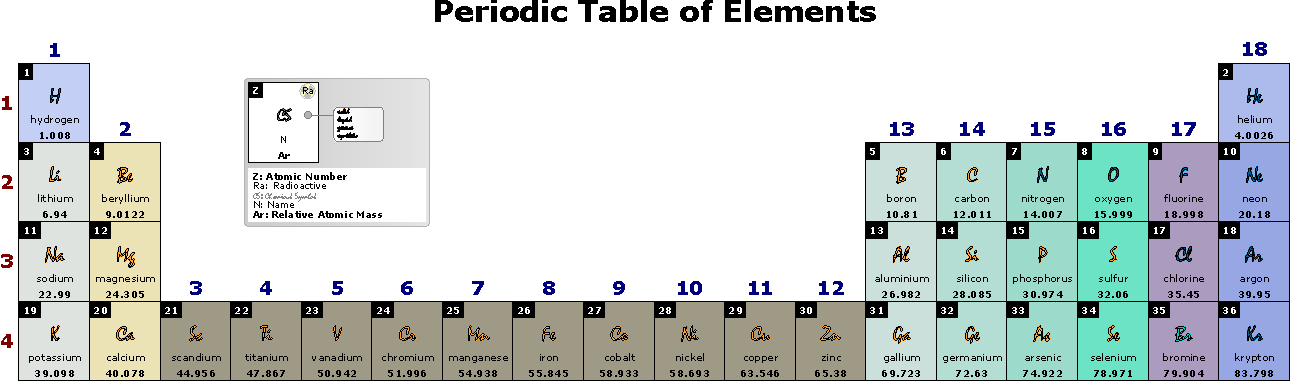
\includegraphics{manualfiles/pgfPTfontLuaXeLaTeX1.pdf}}}%
\newpage
\pgfPTMmacrobox{pgfPT}[Z list={1,...,36},font=Arial,CS font=\string\fontspec{LCALLIG.TTF}\string\selectfont]%
\\ [10pt]\makebox[\linewidth][c]{\scalebox{.6}{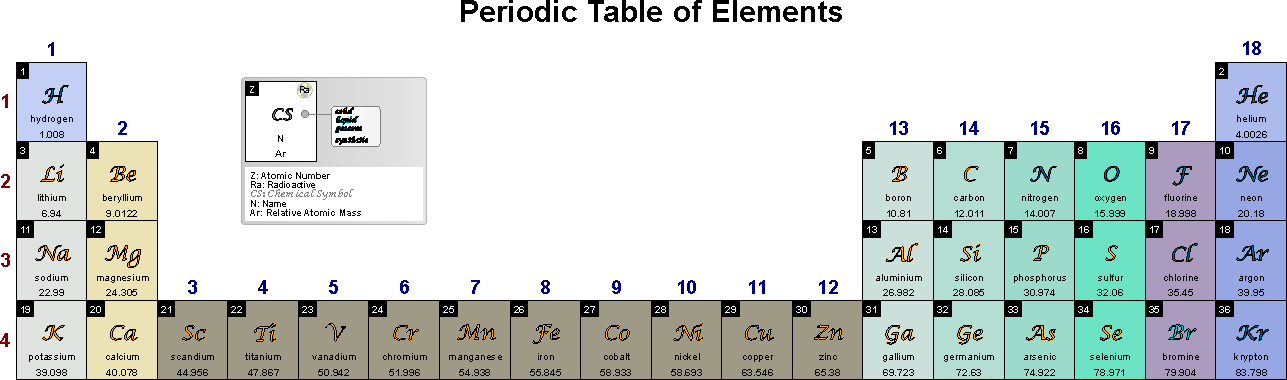
\includegraphics{manualfiles/pgfPTfontLuaXeLaTeX2.pdf}}}%
\\ [5pt]\pgfPTendoption%
% back color scheme
\label{option_back color scheme}%
\vfill
\pgfPTMoption{4}{back color scheme}{pgfPTdefault}%
{Sets a \blue{named} back color scheme for the Periodic Table.}%
\\ [5pt]\pgfPTMmacrobox{pgfPT}[back color scheme=pgfPTSoft]%
\\ [5pt]\makebox[\linewidth][c]{\scalebox{.6}{\pgfPT[back color scheme=pgfPTSoft]}}%
\newpage%
\pgfPTMoptiontxt{%
The possible \lblue{name} is one of the following:
\begin{itembar}
\item\textbf{built-in}:
\begin{itemize}
\item[\raisebox{1pt}{\scriptsize$\vartriangleright\,$}]\sq{pgfPTSoft}, a soft color scheme that distinguishes metals, non metals, silicon and germanium, lanthanoids and actinoids.
\item[\raisebox{1pt}{\scriptsize$\vartriangleright\,$}]\sq{pgfPTJmol}, is the color scheme used in the computer software \href{http://jmol.sourceforge.net/}{Jmol}: an open-source Java viewer for chemical structures in 3D.
\item[\raisebox{1pt}{\scriptsize$\vartriangleright\,$}]\sq{pgfPTCPK}, is the color scheme of the popular color convention for distinguishing atoms of different chemical
elements in molecular models. The scheme is named after the CPK molecular models designed by chemists Robert Corey and Linus Pauling, and improved by Walter Koltun.
\item[\raisebox{1pt}{\scriptsize$\vartriangleright\,$}]\sq{pgfPTRasmol}, is the color scheme used in the computer software \href{http://www.rasmol.org/}{RasMol}, a program for molecular graphics visualization originally developed by Roger Sayle.
\item[\raisebox{1pt}{\scriptsize$\vartriangleright\,$}]\sq{pgfPTRasmolNew}, is a color scheme used in RasMol with revision of CPK colors made by C. Chigbo (RasMol 2.7.3).
\item[\raisebox{1pt}{\scriptsize$\vartriangleright\,$}]\sq{pgfPTWikipedia}, is the color scheme based on the \href{https://en.wikipedia.org/wiki/Periodic_table\#Classification_of_elements}{Wikipedia Periodic Table of Elements}.
\item[\raisebox{1pt}{\scriptsize$\vartriangleright\,$}]\sq{pgfPTMNM}, is designed to show \textbf{M}etals and \textbf{N}on \textbf{M}etals in two different colors, showing also the semi-metals in a third color.
\item[\raisebox{1pt}{\scriptsize$\vartriangleright\,$}]\sq{pgfPTPS}, is designed to show the \textbf{P}hysical \textbf{S}tate of the elements at normal temperature and pressure (NTP) in different colors.
\item[\raisebox{1pt}{\scriptsize$\vartriangleright\,$}]\sq{pgfPTRadio}, is designed to show the \textbf{R}adioactive elements in one color and the non radioactive elements in another color.
\item[\raisebox{1pt}{\scriptsize$\vartriangleright\,$}]\sq{pgfPTBlocks}, for showing the elements in each block of the Periodic Table with the same color.
\item[\raisebox{1pt}{\scriptsize$\vartriangleright\,$}]\sq{solid}, to show the background of each cell of the Periodic Table with the same color specified by the key \sq{\red{back color}}.
\end{itemize}
\item any \textbf{user defined} name via \bs{pgfPTnewColorScheme}\lb\red{name}\rb\lb\red{color list}\rb%
\end{itembar}%
}%
\\ [-5pt]\pgfPTendoption%
% back color
\label{option_back color}%
\pgfPTMoption{4}{back color}{white}%
{Sets the background of each cell of the Periodic Table. It only takes effect if the \red{back color scheme} key is set to \red{solid}}%
\\ [5pt]\pgfPTMmacrobox{pgfPT}[Z list={1,...,36},back color=black!15]%
\\ [10pt]\makebox[\linewidth][c]{\scalebox{.6}{\pgfPT[Z list={1,...,36},back color=black!15]}}%
\\ [10pt]\pgfPTMmacrobox{pgfPT}[Z list={1,...,36},back color scheme=solid,back color=black!15]%
\\ [10pt]\makebox[\linewidth][c]{\scalebox{.6}{\pgfPT[Z list={1,...,36},back color scheme=solid,back color=black!15]}}%
\\ [5pt]\pgfPTendoption%
\newpage\ \vfill%
\textit{It is possible to set the \red{back color scheme} key with the built-in names using the following styles}:\vfill%
% STYLES for back color schemes -> csSoft,csJmol,csCPK,csRasmol,csRasmolNew,csWikipedia,csMNM,csPS,csRadio,csBlocks,csSolid
\label{style_CSchemes}%
\pgfPTMstyle{4}{csSolid}{white}%
{A style equivalent to \red{back color scheme=solid,back color=\#1}}%
\\ [5pt]\pgfPTMmacrobox{pgfPT}[csSolid]%
\\ [10pt]\makebox[\linewidth][c]{\scalebox{.6}{\pgfPT[csSolid]}}%
\\ [10pt]\pgfPTMmacrobox{pgfPT}[csSolid=black!15]%
\\ [10pt]\makebox[\linewidth][c]{\scalebox{.6}{\pgfPT[csSolid=black!15]}}%
\\ [5pt]\pgfPTendstyle%
\newpage\vspace{-34pt}\ %
\foreach \csName/\x in {Soft/0,Jmol/1,CPK/0,Rasmol/1,RasmolNew/0,Wikipedia/1,MNM/0,PS/1,Radio/0,Blocks/1}{%
\pgfPTMstyletxt{4}{cs\csName}{no value}%
{A style equivalent to \red{back color scheme=pgfPT\csName}}%
\\ [5pt]\pgfPTMmacrobox{pgfPT}[cs\csName]%
\\ [10pt]\makebox[\linewidth][c]{\scalebox{.6}{\pgfPT[cs\csName]}}%
\\ [0pt]\pgfPTendstyle%
\ifnum\x=1\relax%
\newpage\vspace{-34pt}\ %
\fi%
}%
% paper (style)
\label{style_paper}%
\pgfPTMstyle{4}{background}{\{\}}%
{A style to set the background of the Periodic Table, built with any of the \txttikz\ keys that can be applied to a path construction.}%
\\ [5pt]\pgfPTMmacrobox{pgfPT}[background={draw=red,line width=2pt,fill=red!10}]%
\\ [10pt]\makebox[\linewidth][c]{\scalebox{.6}{\pgfPT[background={draw=red,line width=2pt,fill=red!10}]}}%
\\ [10pt]\tikz{\node[text width=\linewidth-8pt,inner xsep=4pt,fill=black!10,rounded corners=2pt,font=\small] {\textcolor{black!70}{\textbackslash usetikzlibrary\{shadows\}}};}
\\ [-4pt]\pgfPTMmacrobox{pgfPT}[background={left color=red!10,right color=green!10,postaction={drop shadow={left color=red!10,right color=green!10}}}]%
\\ [10pt]\makebox[\linewidth][c]{\scalebox{.6}{\pgfPT[background={left color=red!10,right color=green!10,postaction={drop shadow={left color=red!10,right color=green!10}}}]}}%
\\ [5pt]\pgfPTendstyle%
% IUPAC
\label{option_IUPAC}%
\pgfPTMoption{4}{IUPAC}{true}%
{When set to true draws the periodic table with \textit{lanthanum} and \textit{actinium} appended to block f and the labels \textit{lanthanoids} and \textit{actinoids} are placed at group 3, substituting \textit{lanthanum} and \textit{actinium}. When \red{IUPAC} is set to false, \textit{lanthanum} and \textit{actinium} are shown in group 3 and the labels \textit{lanthanoids} and \textit{actinoids} are place near the \textit{f block} (if the key \red{show label LaAc} is set to true).
}%
\\ [5pt]\pgfPTMmacrobox{pgfPT}[]%
\\ [10pt]\makebox[\linewidth][c]{\scalebox{.6}{\pgfPT}}%
\\ [10pt]\pgfPTMmacrobox{pgfPT}[IUPAC=false]%
\\ [10pt]\makebox[\linewidth][c]{\scalebox{.6}{\pgfPT[IUPAC=false]}}%
\\ [5pt]\pgfPTendoption%
\newpage\vspace{-34pt}\ %
% show label LaAc
\label{option_show label LaAc}%
\pgfPTMoption{4}{show label LaAc}{\{\}}%
{Determines when the labels \sq{lanthanoids} and \sq{actinoids} are shown (\red{true}) or not shown (\red{false}) near the f block. When the \red{IUPAC} key is set to true, the default behavior is to show the labels and when the \red{IUPAC} key is set to false, the default behavior is to hide the labels. This \textit{default behavior} \textbf{can be overridden by this key} setting it to true, to show the labels, or to false to hide them, independently of the value of the \red{IUPAC} key.
}%
\\ [5pt]\pgfPTMnewZlist{myZlist}{55,...,118}%
\pgfPTnewZlist{myZlist}{55,...,118}%
\\ [-4pt]\pgfPTMmacrobox{pgfPTstyle}[show title=false,show legend=false,show group numbers=false]%
\pgfPTstyle[show title=false,show legend=false,show group numbers=false]%
\\ [-4pt]\pgfPTMmacrobox{pgfPT}[Z list=myZlist]%
\\ [5pt]\makebox[\linewidth][c]{\scalebox{.6}{\pgfPT[Z list=myZlist]}}%
\\ [5pt]\pgfPTMmacrobox{pgfPT}[Z list=myZlist,show label LaAc=true]%
\\ [5pt]\makebox[\linewidth][c]{\scalebox{.6}{\pgfPT[Z list=myZlist,show label LaAc=true]}}%
\\ [5pt]\pgfPTMmacrobox{pgfPT}[Z list=myZlist,IUPAC=false]%
\\ [5pt]\makebox[\linewidth][c]{\scalebox{.6}{\pgfPT[Z list=myZlist,IUPAC=false]}}%
\\ [5pt]\pgfPTMmacrobox{pgfPT}[Z list=myZlist,IUPAC=false,show label LaAc=false]%
\\ [5pt]\makebox[\linewidth][c]{\scalebox{.6}{\pgfPT[Z list=myZlist,IUPAC=false,show label LaAc=false]}}%
\\ [5pt]\pgfPTendoption%
\newpage\vspace{-34pt}\ %
% label LaAc font
\label{option_label LaAc font}%
\pgfPTMoption{4}{label LaAc font}{\string\footnotesize\string\itshape}%
{Sets the font for the labels \sq{lanthanoids} and \sq{actinoids}.}%
\\ [5pt]\pgfPTMmacrobox{pgfPT}[label LaAc font=\string\bfseries,Z list=myZlist,IUPAC=false]%
\\ [10pt]\makebox[\linewidth][c]{\scalebox{.6}{\pgfPT[label LaAc font=\bfseries,Z list=myZlist,IUPAC=false]}}%
\\ [5pt]\pgfPTMmacrobox[l]{pgfPTresetstyle}[]%
\pgfPTresetstyle%
\\ [-10pt]\pgfPTendoption%
% languages
\vfill
\label{option_languages}%
\pgfPTMoption[\pgfPTchangedinversion{2.1.0}]{4}{languages}{\{\}}%
{Sets a language list to use in the Periodic Table. It is a comma separated list of language flags: \sq{pt}, \sq{en}, \sq{fr}, \sq{de}, \sq{it}, \sq{es} or \sq{br}. If a user language has been loaded, the corresponding ISO 639-1 code can also be used as a language flag. \textit{This key locally overrides the default language, that is, the language loaded at package inclusion}.\\ \ }%
\\ [5pt]\pgfPTMmacrobox{pgfPT}[Z list={1,...,36},languages=pt]%
\\ [10pt]\makebox[\linewidth][c]{\scalebox{.6}{\pgfPT[Z list={1,...,36},languages=pt]}}%
\\ [10pt]\pgfPTMmacrobox{pgfPT}[Z list={1,...,36},cell style=pgfPT2lang,languages={en,fr}]%
\\ [10pt]\makebox[\linewidth][c]{\scalebox{.6}{\pgfPT[Z list={1,...,36},cell style=pgfPT2lang,languages={en,fr}]}}%
\newpage%\\ [10pt]
\tikz{\node[text width=\linewidth-8pt,inner xsep=4pt,align=left,fill=black!10,rounded corners=2pt] %
{\small\textcolor{black!50}{\%\ \string\usepackage[userlang=nl]\{pgf-PeriodicTable\}}};}%
\\ [-4pt]\pgfPTMmacrobox{pgfPT}[Z list={1,...,36},cell style=pgfPT2lang,languages={nl,en}]%
\\ [10pt]\makebox[\linewidth][c]{\scalebox{.6}{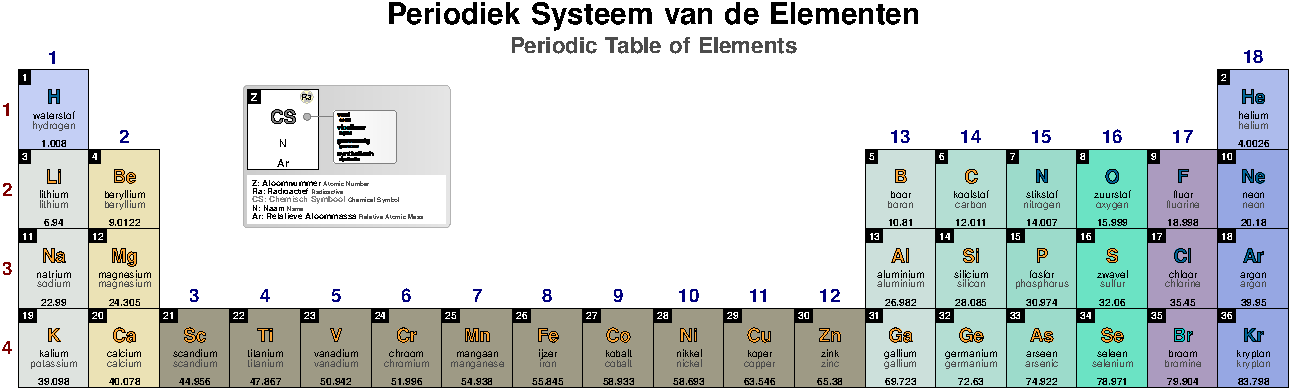
\includegraphics{manualfiles/pgfPT_nl_en.pdf}}}%
\\ [10pt]\pgfPTMmacrobox{pgfPT}[Z list={1,...,36},cell style=pgfPT3lang,languages={pt,fr,it}]%
\\ [10pt]\makebox[\linewidth][c]{\scalebox{.6}{\pgfPT[Z list={1,...,36},cell style=pgfPT3lang,languages={pt,fr,it}]}}%
\\ [10pt]\pgfPTMoptiontxt{%
When using a set of languages, space to accommodate the names in each cell must be provided by building a suitable cell - typically one cell row per language. The cell styles used in the two examples above are built-in and serve this purpose.
\vspace{2.5pt}%
\begin{itembar}
\item\pgfPTpreviewcellstyle[1.5]{pgfPT2lang}\vspace{-10pt}\item\pgfPTpreviewcellstyle[1.5]{pgfPT3lang}
\end{itembar}
\vspace{2.5pt}%
Also, the space for the title should be taken into account -- if using more then three languages, the legend must be \textit{turned off}, otherwise the title overlaps the legend.
}%
\\ [-10pt]\pgfPTendoption%
%\newpage%\vfill%
% other languages font
\label{option_other languages font}%
\pgfPTMoption{4}{other languages font}{\string\tiny}%
{Sets the font used in \textit{other languages}, \ie, the languages started at the second entry of the list provide to the \red{languages} key.}%
\newpage\enlargethispage{\baselineskip}%\\ [5pt]
\pgfPTMmacrobox{pgfPT}[Z list={1,...,36},cell style=pgfPT3lang,languages={en,es,br}, other languages font=\string\tiny\string\bfseries]%
\\ [10pt]\makebox[\linewidth][c]{\scalebox{.6}{\pgfPT[Z list={1,...,36},cell style=pgfPT3lang,languages={en,es,br},other languages font=\tiny\bfseries]}}%
\\ [0pt]\pgfPTendoption%
% other languages color
\label{option_other languages color}%
\pgfPTMoption{4}{other languages color}{black!70}%
{Sets the color of the font used in \textit{other languages}.}%
\\ [5pt]\pgfPTMmacrobox{pgfPT}[Z list={1,...,36},cell style=pgfPT3lang,languages={en,pt,br}, other languages color=purple]%
\\ [10pt]\makebox[\linewidth][c]{\scalebox{.6}{\pgfPT[Z list={1,...,36},cell style=pgfPT3lang,languages={en,pt,br}, other languages color=purple]}}%
\\ [0pt]\pgfPTendoption%
% other lang={f=??,c=??}
\label{style_other lang}%
\pgfPTMstyle{4}{other lang}{\{f=\string\tiny,c=black!70\}}%
{\textit{Pseudo style} to set the keys: other languages \textbf{f}ont and/or other languages \textbf{c}olor. %
None of the \textit{keys} -- f and c -- are mandatory.
\\ [3pt]\makebox[\linewidth][c]{\use{other lang=\{f=<font commands>,c=<color>\}}}%
}%
\\ [5pt]\pgfPTMmacrobox{pgfPT}[Z list={1,...,36},cell style=pgfPT3lang,languages={en,fr,de}, other lang={f=\string\tiny\string\itshape,c=blue}]%
\\ [10pt]\makebox[\linewidth][c]{\scalebox{.6}{\pgfPT[Z list={1,...,36},cell style=pgfPT3lang,languages={en,fr,de}, other lang={f=\tiny\itshape,c=blue}]}}%
\\ [0pt]\pgfPTendstyle%
% show MNM line
\label{option_show MNM line}%
\pgfPTMoption{4}{show MNM line}{true}%
{If set to \red{true} a line separating metals from non metals is shown in the Periodic Table. The line starts at the upper left corner of the cell of boron (2\raisebox{3.5pt}{\footnotesize nd} period, group 13) and ends at the lower right corner of polonium (6\raisebox{3.5pt}{\footnotesize th} period, group 16). If set to \red{false} no line is drawn.
}%
\\ [5pt]\pgfPTMmacrobox{pgfPT}[Z list=spd]%
\\ [10pt]\makebox[\linewidth][c]{\scalebox{.6}{\pgfPT[Z list=spd]}}%
\\ [10pt]\pgfPTMmacrobox{pgfPT}[show MNM line=false]%Z list=spd,
\\ [10pt]\makebox[\linewidth][c]{\scalebox{.6}{\pgfPT[show MNM line=false]}}%Z list=spd,
\\ [10pt]\pgfPTMmacrobox{pgfPT}[Z list={1,...,36}]%
\\ [10pt]\makebox[\linewidth][c]{\scalebox{.6}{\pgfPT[Z list={1,...,36}]}}%Z list=spd,
\\ [0pt]\pgfPTendoption%
%\newpage\vspace{-34pt}\ %
% MNM line color
\label{option_MNM line color}%
\pgfPTMoption{4}{MNM line color}{red!80!black}%
{Sets the color of the \textit{MNM line}.}%
\\ [5pt]\pgfPTMmacrobox{pgfPT}[MNM line color=green]%Z list=spd,
\\ [10pt]\makebox[\linewidth][c]{\scalebox{.6}{\pgfPT[MNM line color=green]}}%Z list=spd,
\\ [0pt]\pgfPTendoption%
% MNM line width
\label{option_MNM line width}%
\pgfPTMoption{4}{MNM line width}{.8pt}%
{Sets the width of the \textit{MNM line}.}%
\\ [5pt]\pgfPTMmacrobox{pgfPT}[MNM line width=1.5pt]%Z list=spd,
\\ [10pt]\makebox[\linewidth][c]{\scalebox{.6}{\pgfPT[MNM line width=1.5pt]}}%Z list=spd,
\\ [0pt]\pgfPTendoption%
% MNM={c=??,w=??} (pseudo style)
\label{style_MNM}%
\pgfPTMstyle{4}{MNM}{\{c=red!80!black,w=.8pt\}}%
{\textit{Pseudo style} to set the \textit{MNM line} \textbf{c}olor and/or \textbf{w}idth. None of the \textit{keys} -- c and w -- are mandatory. The key \red{show MNM line} is set to \red{true}.
\\ [3pt]\makebox[\linewidth][c]{\use{MNM=\{c=<color>,w=<length>\}}}%
}%
\\ [5pt]\pgfPTMmacrobox{pgfPT}[MNM={w=1.5pt,c=red}]%Z list=spd,
\\ [10pt]\makebox[\linewidth][c]{\scalebox{.6}{\pgfPT[MNM={w=1.5pt,c=red}]}}%Z list=spd,
\\ [0pt]\pgfPTendstyle%
\endinput%
